\chapter{粒子、波、および分解能のエネルギー}

\section{粒子か場か？}

素粒子物理学とは何を扱うのか。粒子---だが、その答えは直ちに古くからの問いを呼び起こす。自然は離散的だろうか。ここで離散的とは、物質が分離した不可分の単位からなるということであり、角が立たないという意味ではない。ギリシア語の\emph{アトム}は不可分を意味するが、現在アトムと呼ばれる物体は分割できる。当面、\emph{粒子}を離散的な単位の総称とする。

対立する描像は連続体である。その場合、物質は分離した断片の集まりではなく、空間を通じて連続的に広がるものである。その自然な言語は場の言語である。場とは位置の関数である。物質の密度は場であり、電場と磁場も場である。後者は荷電粒子がどのように運動するかを決めるが、場それ自体は古典的には空間に連続的に分布するものとして考えられる。

これらの考えの歴史的順序はあまり厳密に押し付けるべきではない。この順序が有用なのは、議論の論理を示すからであり、信頼できる年代順を与えるからではない。粒子の語彙には原子、分子、衝突、局在した物体が含まれ、連続体の語彙には場と連続的に変化する性質が含まれる。どちらの描像が正しいのか。量子力学はどちらも完全に正しいことを妨げるが、どちらも完全に誤りであることも妨げる。

以下の議論は部分的には自己完結的であるが、後の議論では量子力学、古典力学、特殊相対性理論、電磁気学を利用する。当面の問いはもっと単純である。物質が本当に離散的であると人々を最初に納得させたのは何か。

\section{離散的物質の化学的証拠}

少なくともこの論理的な説明では、最初の真剣な証拠は物理学ではなく化学から来た。この区別は人為的である。化学は大部分が原子と分子の物理学である。ドルトンは異なる物質の同数の分子の質量を比較した。試料が同数の分子を含むことを確立すること自体が大きな問題であった。ここでアボガドロの名が登場し、モルはアボガドロ数個の分子である。同じ数の分子を含む試料を比較するだけなら、その数の実際の値は必要なかった。

目覚ましいパターンは、モル質量が水素のモル質量のほぼ整数倍で現れることであった。その倍数は一般に\(3/2\)や\(\pi\)や任意の実数ではなく、整数に近い数であった。例えば炭素-12は、水素が表す質量単位をおよそ12個持つ。これはほぼ同じ質量の反復する構成要素からできていることを強く示唆する。

現代的な説明はこの謎を取り除く。通常の原子には陽子、中性子、電子が含まれている。電子の質量は陽子や中性子のわずか約二千分の一にすぎないため、電子が原子質量に寄与する割合は小さい。陽子と中性子がそのほとんどすべてを担っており、両者の質量の差は一パーセントよりはるかに小さい。通常の水素の原子核は陽子一個であるから、原子や分子の質量は水素程度の核質量のほぼ整数倍となる。この記述はあくまで近似的である。陽子と中性子の質量は同一ではなく、電子もわずかに寄与する。それでもなお、このほぼ整数倍という規則性は離散的な構成要素の存在を明らかにしている。

その後、分子は原子の組み合わせとして理解された。19世紀の化学はおよそ100種類の原子を同定し、それらを元素として整理した。初等的な数え方ではおよそ92種類が天然に存在し、同位体を含めるとさらに区別が増える。周期表は等しいブロックを単純に繰り返すという素朴な意味での周期的ではないが、それらの別個の種を整理した。その段階では、元素それ自体が基本的な構成要素のように見えた。アインシュタインの1905年の仕事は、物質の分子論をはるかに決定的に確立する定量的な方法を与えたが、化学的証拠はすでに原子描像を説得力のあるものにしていた。

19世紀の終わり近くに、この見かけ上の終着点は破綻した。電子が発見され、放射能は元素が基本的であるという描像に収まらない現象を明らかにした。放射能は、後に核物理学と素粒子物理学となる多くの問いを、すでに縮図として内包していた。

\section{放射能と分離されたビーム}

正確な帰属と年代順は不確かである。ベクレルは、放射性物質がたまたま写真乾板の近くにあり、あたかも不可視の放射線がそれを照射したかのように乾板に影響を与えたという観察と暫定的に関連づけられている。かぶった乾板を単に台無しになったものとして扱うのではなく、そこに何が到達したのかを問うこともできた。マリー・キュリーのその後の広範な研究もまたこの歴史に属するが、初期の発見の正確な分担は、この実験的論理には必要ない。

物質を密な鉛ブロックの深部に置き、写真乾板へ向かう細い通路を残す。鉛は密度が高いため有用であり、通路は逃げ出すものをコリメートする。拡散した露光ではなく、乾板には局所的な斑点が現れ、指向性のあるビームを示唆する。この論理的な意味でそれは最初の粒子ビームであるが、この段階ではビームの本性は不明である。

次に、コリメートされた放射を、軌道の平面に垂直な磁場に通す。露光は三つの枝に分かれる。一つは偏向されずに進む。二つは逆向きに曲がり、しかも不等な量だけ曲がる。磁気力は電荷の符号が逆になると向きが逆になるので、逆向きに曲がった枝は逆向きに帯電した放射として振る舞い、直進する枝は中性の放射として振る舞う。\footnote{模式図は、講義動画において00:14:34と00:19:31の間に展開された図を再構成したものである。}

\begin{figure}[h]
\centering
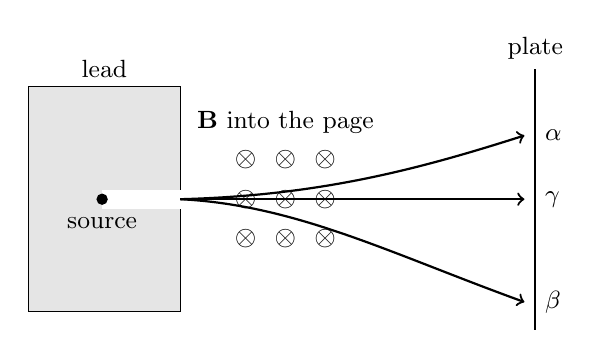
\begin{tikzpicture}[scale=0.92]
\draw[fill=gray!20] (0,-1.55) rectangle (2.1,1.55);
\draw[fill=white,draw=none] (1.02,-0.13) rectangle (2.12,0.13);
\draw[fill=black] (1.02,0) circle (0.07);
\node[below] at (1.02,-0.12) {\small source};
\node[above] at (1.05,1.55) {\small lead};
\foreach \x in {3.0,3.55,4.1}
  \foreach \y in {-0.55,0,0.55}
    \node at (\x,\y) {\(\otimes\)};
\node[above] at (3.55,0.78) {\small \(\mathbf B\) into the page};
\draw[thick] (7,-1.8) -- (7,1.8);
\node[above] at (7,1.8) {\small plate};
\draw[thick,->] (2.1,0) -- (6.85,0);
\draw[thick,->] (2.1,0) .. controls (4.0,0.05) and (5.35,0.40) .. (6.85,0.88);
\draw[thick,->] (2.1,0) .. controls (3.7,-0.08) and (5.0,-0.75) .. (6.85,-1.42);
\node[right] at (7,0.88) {\small \(\alpha\)};
\node[right] at (7,0) {\small \(\gamma\)};
\node[right] at (7,-1.42) {\small \(\beta\)};
\end{tikzpicture}
\caption{横方向の磁場中にあるコリメートされた放射性ビーム。中性成分は偏向されず、逆向きに帯電した成分は不等な量だけ逆向きに曲がる。}
\end{figure}

三つの成分はアルファ、ベータ、ガンマと名づけられた。現代的な用語では、
\begin{equation}
\begin{aligned}
\beta\text{-radiation} &= \text{electrons},\\
\alpha\text{-radiation} &= \text{helium nuclei},\\
\gamma\text{-radiation} &= \text{photons}.
\end{aligned}
\end{equation}
アルファ粒子は二つの陽子と二つの中性子を含み、その質量数四を説明する。ドルトンの近似的な整数の系列では、ヘリウムはしたがって番号四を占めることになる。すなわち四つの水素スケールの核単位である。ベータ線は、陰極線実験からすでに知られていた負に帯電した電子である。ガンマ線は電荷を運ばない。

十分に希薄な線源と、個々の到来を分解できる検出器を用いれば、連続的に見える露光は別々の事象の列になる。ブリップ、ブリップ、ブリップ。同じことはベータ線、アルファ線、ガンマ線についても行える。ガイガー計数管は、最も初期の装置がまさにその領域で操作されていたかどうかにかかわらず、正しい描像を与える。各成分は離散的な束として到来する。ガンマは依然として謎である。それは中性であるのに、一度に一つの事象として検出される。ガンマ線は非常に高エネルギーの光であり、プランク、とりわけアインシュタインは光を量子と結びつけた。しかし、その結論に立ち向かう前に、光が波であるという古典的な証拠を真剣に受け止めなければならない。

\section{光の古典的波動性}

古典的には、光は連続性の最も強い例であった。それは連続的な波として伝播する電場と磁場からなる。ニュートンは粒子説を好んだが、波動の実験がそれを退けた。電荷を揺さぶると電磁放射が生じる。巨視的なアンテナは電波、マイクロ波、赤外線、可視光、または紫外線を放出でき、原子内を回る電荷もまたアンテナである。放出された放射は写真乾板を露光させうる。

単一の開口は波動的振る舞いの最初の兆候を与える。もし光が弾丸の流れであれば、小さな開口は鋭くコリメートされた斑点を作ると予想される。そうではなく、照明はぼやけた領域に広がる。しかし、広がりだけでは決定的ではない。なぜなら、粒子が開口の縁の力によって偏向されると想像することもできるからである。

二つの開口はより鋭い試験を与える。二つの独立な粒子の流れは二つの重なり合うにじみを与え、おそらく重なる場所で最も明るくなるであろう。波は異なることをする。一方の開口からの山は他方からの山と出会って強め合うことができる。山は谷と出会って打ち消し合うこともできる。したがってスクリーンには明暗の縞が交互に現れ、どちらか一方の開口だけなら照明するであろう暗い場所も含まれる。\footnote{模式図は、講義動画において00:25:00と00:29:49の間に展開された開口と干渉の図を再構成したものである。}

\begin{figure}[h]
\centering
\resizebox{\linewidth}{!}{%
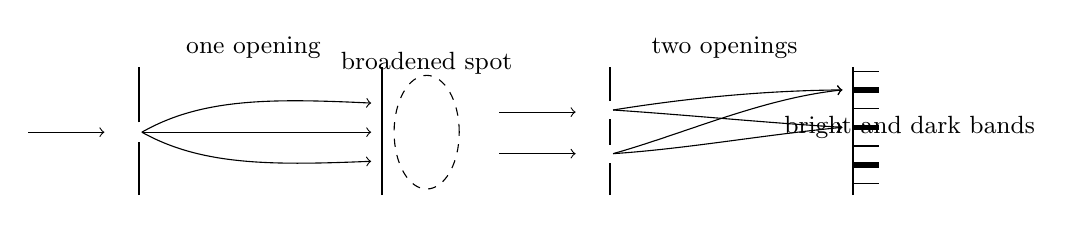
\begin{tikzpicture}[scale=0.88]
\begin{scope}
\draw[->] (-0.3,1.06) -- (0.8,1.06);
\draw[thick] (1.3,0.15) -- (1.3,0.92);
\draw[thick] (1.3,1.20) -- (1.3,2.0);
\draw[thick] (4.8,0.15) -- (4.8,2.0);
\draw[->] (1.34,1.06) .. controls (2.2,1.55) and (3.2,1.55) .. (4.65,1.48);
\draw[->] (1.34,1.06) -- (4.65,1.06);
\draw[->] (1.34,1.06) .. controls (2.2,0.58) and (3.2,0.58) .. (4.65,0.64);
\draw[dashed] (5.45,1.06) ellipse (0.47 and 0.82);
\node at (2.95,2.28) {\small one opening};
\node at (5.45,2.05) {\small broadened spot};
\end{scope}
\begin{scope}[xshift=6.8cm]
\draw[->] (-0.3,1.35) -- (0.8,1.35);
\draw[->] (-0.3,0.75) -- (0.8,0.75);
\draw[thick] (1.3,0.15) -- (1.3,0.62);
\draw[thick] (1.3,0.88) -- (1.3,1.25);
\draw[thick] (1.3,1.51) -- (1.3,2.0);
\draw[thick] (4.8,0.15) -- (4.8,2.0);
\draw[thin] (4.8,0.32) -- (5.18,0.32);
\draw[line width=2pt] (4.8,0.59) -- (5.18,0.59);
\draw[thin] (4.8,0.86) -- (5.18,0.86);
\draw[line width=2pt] (4.8,1.13) -- (5.18,1.13);
\draw[thin] (4.8,1.40) -- (5.18,1.40);
\draw[line width=2pt] (4.8,1.67) -- (5.18,1.67);
\draw[thin] (4.8,1.94) -- (5.18,1.94);
\draw[->] (1.34,0.75) .. controls (2.4,0.82) and (3.5,1.02) .. (4.65,1.13);
\draw[->] (1.34,1.38) .. controls (2.4,1.31) and (3.5,1.20) .. (4.65,1.13);
\draw[->] (1.34,0.75) .. controls (2.4,1.05) and (3.5,1.55) .. (4.65,1.67);
\draw[->] (1.34,1.38) .. controls (2.4,1.55) and (3.5,1.66) .. (4.65,1.67);
\node at (2.95,2.28) {\small two openings};
\node at (5.62,1.13) {\small bright and dark bands};
\end{scope}
\end{tikzpicture}
}
\caption{単一の開口は広がった像を生じ、二つの開口は交互の建設的および破壊的干渉を生じる。}
\end{figure}

同じ効果は水でも容易に想像できる。水面に二本の指を揺らしてみよ。円形の波が広がり、ある場所では強め合い、別の場所では打ち消し合う。単なる広がりではなく、干渉こそが決定的な波の特徴である。

歴史的な順序もまた単純ではない。この概略的な説明では、ホイヘンスは波の伝播の提唱者としてニュートンの前に置かれ、トマス・ヤングは干渉の実証と結び付けられ、ニュートン自身の光学実験のいくつかは、彼が粒子説を支持していたにもかかわらず、波の干渉による解釈を許容する。その後の干渉実験は、光の波動性を合理的な疑いの余地なく確立した。

次にマクスウェルは、何が振動しているのかを突き止めた。光波がある軸に沿って伝播するなら、その電場はその軸に垂直である。その磁場もまた垂直であり、電場に対して直交している。この完全なパターンは光速で進む。\footnote{模式図は講義動画の00:31:08で描かれた電磁波の図を再構成したものである。}

\begin{figure}[h]
\centering
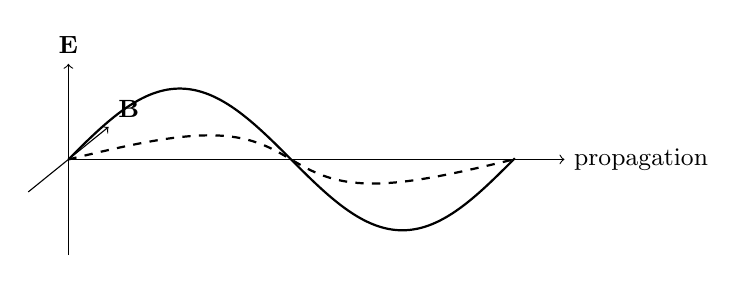
\begin{tikzpicture}[
  scale=0.9,
  x={(1cm,0cm)},
  y={(0cm,1cm)},
  z={(0.42cm,0.34cm)}
]
\draw[->] (0,0,0) -- (7,0,0) node[right] {\small propagation};
\draw[->] (0,-1.35,0) -- (0,1.35,0) node[above] {\small \(\mathbf E\)};
\draw[->] (0,0,-1.35) -- (0,0,1.35) node[above right] {\small \(\mathbf B\)};
\draw[thick,smooth,variable=\x,domain=0:6.3,samples=100]
  plot ({\x},{sin(\x r)},0);
\draw[thick,dashed,smooth,variable=\x,domain=0:6.3,samples=100]
  plot ({\x},0,{sin(\x r)});
\end{tikzpicture}
\caption{電磁波では、電場と磁場は互いに直交し、どちらも伝播方向に対して垂直である。}
\end{figure}

通常の可視光はあまりにも速く振動するため、その交互に変わる場を直接追跡することはできない。極端に長い電波では、振動はそれに対応して遅くなる。いずれの場合も、同じ横波の幾何学が干渉をもたらす。

\section{波長、周期、振動数}

波長\(\lambda\)は空間的な距離である。振動のある点から出発し、一波長の周期の後に同じ位相が再び現れるまで波に沿って進む。それはメートル、センチメートル、その他の長さの単位で測られる。

次に、波が通過する間、一つの位置に立ってみよ。一つの完全な周期に要する時間が周期\(T\)である。可視光の周期は極めて短く、およそ\(10^{-15}\,\mathrm{s}\)の程度である。より長い波長はより長い周期に対応し、より短い波長はより短い周期に対応する。

一周期の間に波は一波長だけ進むので、速さ\(v\)の波は次を満たす。
\begin{equation}
v=\frac{\lambda}{T}.
\end{equation}
水波や音波にはそれぞれ固有の伝播速度がある。光については、
\begin{equation}
c=\frac{\lambda}{T}.
\end{equation}
振動数\(f\)は単位時間あたりの周期の数である。
\begin{equation}
f=\frac{1}{T}.
\end{equation}
したがって
\begin{equation}
\lambda f=c.
\end{equation}
波長か振動数のどちらかが他方を決定する。

\begin{figure}[h]
\centering
\includegraphics[width=0.68\textwidth]{lecture_01_figure_03.png}
\caption{光波については、\(f=1/T\)および\(\lambda f=c\)である。}
\lectureframe{00:36:24}
\end{figure}

物理学者は、一秒あたりの完全な周期の数ではなく、一秒あたりのラジアンで振動の速さを測ることが多い。円周に沿った等速運動を想像してみよ。その点が毎秒\(f\)回転し、各回転が\(2\pi\)ラジアンを含むなら、その角振動数は
\begin{equation}
\omega=2\pi f,
\qquad
\frac{\omega}{2\pi}=f.
\end{equation}
今のところこれは定義である。これが\(2\pi\)の因子の数を減らすかどうかという実用的な問題は、後で戻ってくる。

\(f=c/\lambda\)と\(\omega=2\pi f\)を組み合わせると
\begin{equation}
\omega=\frac{2\pi c}{\lambda},
\qquad
\omega\lambda=2\pi c.
\end{equation}
別の種類の波では、\(c\)はその波の伝播速度に置き換えられる。

\begin{figure}[h]
\centering
\includegraphics[width=0.68\textwidth]{lecture_01_figure_04.png}
\caption{\(\omega=2\pi f\)のもとで、光波は\(\omega=2\pi c/\lambda\)を満たす。}
\lectureframe{00:39:10}
\end{figure}

電磁放射は連続的なスペクトルを形成する。長い波長から短い波長へと並べると、従来の名称は次のとおりである。
\begin{equation}
\begin{aligned}
\text{radio}
&\longrightarrow \text{microwave}
\longrightarrow \text{infrared}
\longrightarrow \text{visible}\\
&\longrightarrow \text{ultraviolet}
\longrightarrow \text{X ray}
\longrightarrow \text{gamma ray}.
\end{aligned}
\end{equation}
可視光は狭い間隔を占めるにすぎない。名付けられた領域の境界は慣習的なものであるため、ここでは正確な分割波長は必要ない。電波は極端に長くなりうる。ガンマ線は電磁スペクトルの非常に短い波長の端である。ここで困難は鋭くなる。ガンマ線は古典的には連続的な場の波であるが、離散的なパルスとして検出される。

\section{離散的な到来と波の確率}

放射の熱力学的性質は、プランクとアインシュタインを、光は離散的な単位で扱わなければならないという結論へと導いた。想像上の実験はこの点を鮮明にするが、それは発見に至った実際の歴史的経路についての主張ではない。

スクリーンにビームを当てる。通常の強度では、連続的に見える明るい斑点ができる。ビームに部分的に不透明な減衰器を入れると、斑点は暗くなる。減衰を繰り返し増やすと、単位時間あたりに届く光は少なくなる。やがて見え方が変わる。連続的に暗い斑点ではなく、検出器は孤立した事象を記録する。\footnote{模式図は講義動画の00:42:32と00:45:42の間で展開された減衰実験を再構成したものである。}

\begin{figure}[h]
\centering
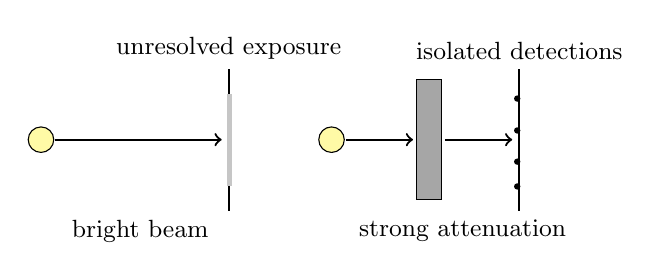
\begin{tikzpicture}[scale=0.9]
\begin{scope}
\draw[fill=yellow!35] (0,0) circle (0.18);
\draw[->,thick] (0.2,0) -- (2.55,0);
\draw[thick] (2.65,-1.0) -- (2.65,1.0);
\node[below] at (1.4,-1.0) {\small bright beam};
\end{scope}
\begin{scope}[xshift=4.1cm]
\draw[fill=yellow!35] (0,0) circle (0.18);
\draw[->,thick] (0.2,0) -- (1.15,0);
\draw[fill=gray!70] (1.2,-0.85) rectangle (1.55,0.85);
\draw[->,thick] (1.6,0) -- (2.55,0);
\draw[thick] (2.65,-1.0) -- (2.65,1.0);
\node[below] at (1.85,-1.0) {\small strong attenuation};
\end{scope}
\fill[gray!45] (2.62,-0.65) rectangle (2.70,0.65);
\foreach \y in {-0.66,-0.31,0.13,0.58}
  \fill (6.72,\y) circle (0.045);
\node[above] at (2.65,1.0) {\small unresolved exposure};
\node[above] at (6.75,1.0) {\small isolated detections};
\end{tikzpicture}
\caption{漸進的な減衰は検出率を下げ、連続的に見える露光が孤立した光子事象へと分解される。}
\end{figure}

十分に長く待てば、それらの事象は元の塊と同じ空間的プロファイルへと蓄積される。したがって明るい領域は、多数の個々の到達の分解されていない総和であった。この低強度の実験は実行可能であるが、もともと光子仮説を動機づけた初期の実験ではなかった。アインシュタインの光子提案は熱力学と光電効果の考察から生じたものであり、減衰実験はその帰結を描くための特に直接的な方法を与える。

次に、ビームに二つの開口を置き、光子が一度に一つずつ到着するまで強度を下げる。各検出は局在したブリップである。しかし多くの検出の後、ブリップは明帯と暗帯を含む干渉縞を埋め尽くす。離散的な到達はランダムであるが、その確率分布は波動パターンが予測する分布である。古典的な波は、確率を支配する波になったのである。

したがって、波と粒子は、自然の異なる部分に割り当てられた二種類の別個の実体ではない。それらは同一の量子対象の二つの現れである。光は、波だけ、あるいは粒子だけとして十分に記述することはできない。

電子は当初の驚きを逆転させる。電子は粒子として受け入れられ、検出器に一度に一つずつ到着するが、十分に近い開口を用いれば、同様に干渉縞を形成する。電子の約八千倍の質量をもつアルファ粒子も同じ原理に従うが、実験はより難しい。干渉はバッキーボールでも観測されている。すなわち、およそ一般化されたサッカーボールのように配置された六十個の炭素原子からなる分子である。同じ原理はボウリング球にも当てはまると予想されるが、そのような実験は途方もなく非現実的である。議論は、ますます野心的な例として、ウイルスや生きた細胞を用いた提案実験へと押し進めることができる。波と粒子の記述がどのように整合するかを理解するには量子力学が必要であるが、当面の課題は素粒子物理学に必要な光子の性質を引き出すことである。

\section{光子のエネルギー}

光子は光の離散的で不可分な要素である。光はエネルギーを運ぶ---太陽光は吸収体を加熱する---ので、各光子はエネルギーを運ばなければならない。単色波は確定した波長と角振動数をもち、その中のすべての光子は
\begin{equation}
E_\gamma=\hbar\omega.
\end{equation}
連続的な波を小さな力学的な点の集まりとして思い描こうとするのは誤解を招く。確定しているのは実験的な組み合わせである。局在した検出は波に支配された分布で起こり、エネルギーは不可分な単位で到着する。

\begin{equation}
\omega=\frac{2\pi c}{\lambda},
\end{equation}
であるから、より短い波長はより大きな角振動数を意味し、したがって各光子により大きなエネルギーをもたらす：
\begin{equation}
\lambda\downarrow
\quad\Longrightarrow\quad
\omega\uparrow
\quad\Longrightarrow\quad
E_\gamma\uparrow.
\end{equation}
単一の電波光子はごくわずかなエネルギーしかもたない。それでも電波ビームは、非常に多くの光子を含むことによって莫大な全エネルギーを運ぶことができる。\(n\)個の光子を含む単色パルスに対して、
\begin{equation}
E_{\text{pulse}}=n\hbar\omega,
\qquad
n=0,1,2,\ldots.
\end{equation}
総量は大きくてもよいが、それは一光子エネルギーの整数倍にとどまる。

この関係は、残りの議論を支配することになる実用的な問いへと導く。なぜ、より小さくより小さなものを見るために、より大きくより大きな機械を造らなければならないのか。なぜ小さな対象に小さな機械を使わないのか。答えの前半はすでに述べられている。より小さな構造を分解するにはより短い波長が必要であり、より短い波長の量子はより大きなエネルギーを運ぶのである。

\section{静止エネルギーと不変質量}

素粒子物理学は量子力学と相対性理論を組み合わせる。光子の関係\(E_\gamma=\hbar\omega\)は量子側を与え、相対性理論からの対応する初等的な事実は
\begin{equation}
E_{\mathrm{rest}}=mc^2.
\end{equation}
この限定は重要である。古い説明では\emph{静止質量}を、速度に依存する\emph{運動質量}から区別していた。現代の用語では\emph{質量}を対象の不変質量に対して用いる。運動はそのエネルギーを変えるが、質量は変えない。すべての電子は、その運動状態が何であれ同じ質量をもつ一方、電子のエネルギーは加速されるにつれて増大する。したがって\(E=mc^2\)は、この形では、対象全体が静止している基準系における質量をもつ対象のエネルギーである。

対象は内部的に静止している必要はない。気体の箱は、その分子が四方八方に速く運動していても、秤の上で静止していられる。それらの内部運動のエネルギーは、完全な箱の静止エネルギーの一部である。冷たい箱から始めてその質量を測定し、次に箱自体を静止させたまま熱エネルギーを加える。その静止質量は
\begin{equation}
\Delta m=\frac{\Delta E_{\mathrm{internal}}}{c^2}.
\end{equation}
だけ変化する。その重さと慣性は質量とともに増大する。普通の箱では、大きな温度上昇の後でさえ、その効果は普通の秤では気づかないほど小さすぎる。効果の小ささは原理を変えるものではない。

より鮮明な例として、電子と陽電子を用いる。両者は質量が正確に等しく、電荷が反対である。それらが最初静止しており、対消滅すると、光子がエネルギーを持ち去る：
\begin{equation}
e^-+e^+\longrightarrow \text{photons}.
\end{equation}
初期エネルギーは
\begin{equation}
E_{\mathrm{initial}}=2m_e c^2,
\end{equation}
であり、そのエネルギーは消えることができない。一対から得られるのはごくわずかであるため、一杯のコーヒーを温めるにさえ膨大な数の対が必要であろうが、個々の対消滅事象はこの変換を直接示す。

したがって、静止している物体にとって、質量とエネルギーは異なる単位で表された同じ物理量である。因子\(c^2\)は、慣用の質量単位とエネルギー単位の間の換算因子であり、ちょうど数値因子がメートルをセンチメートルに換算するのとよく似ている。

\begin{classroomqa}
\lecturetimestamp{01:04:39}
\audiencequestion{質量を放出エネルギーに変換するには機構が必要なのか。}
\lecturerresponse{はい、物理的機構が必要であるが、保存則はすでにその結果を制約している。微視的な対消滅機構が記述される前でさえ、初期の電子--陽電子のエネルギーはどこかに再び現れなければならない。したがって、エネルギー保存則は、相互作用の詳細な説明なしに、答えの重要な部分を決定することができる。}
\end{classroomqa}

\section{次元と単位の選択}

SI単位では、光速は非常に大きな数であり、プランク定数は非常に小さな数である。後者の小ささは、すでに光子の関係式によって示唆されている。可視光の角振動数は膨大である一方、一光子のエネルギーはごくわずかであるため、\(E_\gamma=\hbar\omega\)はこれらの単位において\(\hbar\)の小さな数値を必要とする。桁の程度では、
\begin{equation}
c\sim 10^8\ \mathrm{m\,s^{-1}},
\qquad
\hbar\sim 10^{-34}\ \mathrm{J\,s}.
\end{equation}
\editorialnote{最終的な板書の数字が不明瞭であるため、講義で述べられた桁の程度のみを保持している。}
単位は不可欠である。どちらの定数も単なる裸の小数ではない。エネルギーは次元
\begin{equation}
[E]=M L^2 T^{-2},
\end{equation}
を持ち、\(E_\gamma=\hbar\omega\)で\([\omega]=T^{-1}\)であるから、プランク定数は次元
\begin{equation}
[\hbar]=[E]T=M L^2 T^{-1}.
\end{equation}
を持つ。

\(c\)が大きく\(\hbar\)が小さいと呼ぶこと自体、すでに単位の選択を前提としている。速さをフィート毎時で測れば、メートル毎秒で測るのとは異なる\(c\)の数値が得られる。光年毎年、あるいは光秒毎秒では、光速は単に1である。質量、長さ、時間の単位を適切に協調して選べば、同様に\(\hbar=1\)とすることができる。

おなじみの単位系は受け継がれた慣習であり、自然に特権的に備わった特徴ではない。一マイルは5280フィートを含み、一ストーンは十四ポンドを含み、馬はハンドで測られ、動力は馬力で測られることがある。メートル法の単位はより体系的であるが、その目盛りは依然として人間の選択である。基礎物理学のうちに、メートル、秒、キログラムを特に選び出すものは何もない。

長さ、時間、質量は三つの独立な基本単位の選択を与える：
\begin{equation}
L,\qquad T,\qquad M.
\end{equation}
他の力学的単位はこれらから構成できる。有用な選択は問題に依存する。太陽質量は天体物理学で便利であり、陽子質量は核物理学で便利であろう。光年と年は相対論的天文学の公式を簡潔にする。三つの独立な選択があれば、三つの独立な次元定数に都合のよい数値を割り当てることができる。天体物理学、原子物理学、素粒子物理学は同じ選択をする必要はない。

素粒子物理学にとって、特に有用な二つの規約は
\begin{equation}
c=1,
\qquad
\hbar=1.
\end{equation}
である。残りの単位については、同程度に際立った粒子質量は存在しない。陽子質量、ヒッグス粒子質量、あるいはミューオン質量を1と宣言することもできるが、それは大きな集合の一員を特権化するにすぎない。

では、なぜ\(c\)と\(\hbar\)を選ぶのか。第一の答えは、それらが多くの方程式に現れるからかもしれない。出現頻度だけでは十分でない。陽子質量も多くの方程式に現れ、陽子の大きさも同様である。\(c\)と\(\hbar\)を際立たせるのは、それらの普遍性である。

定数\(c\)と\(\hbar\)は異なる。速さ\(c\)はあらゆる物理的物体を制約する。質量をもつ物体はそれに近づくことはできるが、それを超えて加速されることはできない。プランク定数は、桁の程度の不確定性関係
\begin{equation}
\Delta x\,\Delta p\gtrsim\hbar.
\end{equation}
を通じてあらゆる量子物体を制約する。どちらの言明も特定の種類の粒子を選び出すものではない。この普遍性が、\(c=1\)と\(\hbar=1\)を自然な規約とするのである。

陽子は同程度に普遍的な尺度を与えない。それは多くの物体のうちの一つにすぎない。陽子質量を1とすることは、ルビジウム原子の質量を1とすること以上に根本的な地位をもたない。電子、ヒッグス粒子、ミューオンも同じ困難を示す。

電荷は別の普遍的な量を示唆するが、\(c\) と \(\hbar\) を規格化した後では、物理的に重要な電磁結合は無次元である。単位を変えれば、電磁気の式の周りで次元を持つ定数を動かすことはできるが、真に無次元の結合を変えることはできない。

重力は次元を持つ普遍定数を与える。ニュートン形式では、二つの質量の間にはたらく力の大きさは
\begin{equation}
F=G\frac{m_1m_2}{r^2}.
\end{equation}
である。すべての質量は重力を及ぼすが、電気的に中性な物体は電気力に関与する必要はない。したがって \(G\) は要求される普遍性を備えている。それにもかかわらず、通常の素粒子物理学にとって実用的な規格化としては不適切である。なぜなら、既知の素粒子の間の重力は、ここで議論している計算では無視できるからである。

\begin{classroomqa}
\lecturetimestamp{01:20:34}
\audiencequestion{単に \(G\) を無視することは正当だろうか。非常に高いエネルギーでは、素粒子は仮定されているような仕方で古典重力に従わないかもしれない。}
\lecturerresponse{個々の粒子は実際に地球の重力場に応答する。すなわち、単一の粒子はその場の中で落下する。一方の素粒子が他方に及ぼす重力的影響は直接測定されていないため、そのレベルでは普遍性の仮定は疑問視されうる。\(G\) を除外しておく直接の理由は、絶対的なものではなく実用的なものである。重力は通常の素粒子物理学の実験や方程式には無視できるほどしか寄与しない。}
\end{classroomqa}

\begin{classroomqa}
\lecturetimestamp{01:22:01}
\audiencequestion{重力の代わりに、電気相互作用を第三の単位設定の規約として用いることはできるだろうか。}
\lecturerresponse{できる。電荷、またはクーロンの法則に現れる定数を規格化する電磁単位を選ぶことができる。そのような規約は用いられている。電子は引き合うのではなく反発するが、その符号はこの選択を妨げない。それは単にここで採用されている規約ではないだけである。}
\end{classroomqa}

\begin{classroomqa}
\lecturetimestamp{01:23:06}
\audiencequestion{\(c\) と \(\hbar\) を 1 に等しいと置くと、電荷は無次元になるだろうか。}
\lecturerresponse{はい。電荷の二乗に関連する無次元の尺度はおよそ \(1/137\) である。正確な規約とその数の意味は後回しにしてよい。ここでの要点は、それが無次元であるということである。}
\end{classroomqa}

\begin{classroomqa}
\lecturetimestamp{01:23:37}
\audiencequestion{クーロン定数を、1 に等しいと置く第三の定数として選ぶことはできるだろうか。}
\lecturerresponse{それは電磁単位の規約に吸収することができる。その選択によって無次元の結合 \(1/137\) を 1 に変えることはできない。なぜなら、単位を変えても無次元の数を変えることはできないからである。ここでその規約を採用することに特に利点があるとは主張しない。}
\end{classroomqa}

\section{自然単位の方程式と基準系}

\(c=1\) のもとでは、質量をもつ物体の静止エネルギー関係は
\begin{equation}
E_{\mathrm{rest}}=m.
\end{equation}
となる。\(\hbar=1\) のもとでは、光子の関係は
\begin{equation}
E_\gamma=\omega.
\end{equation}
となる。従来の単位での数値的な大きさが必要なときはいつでも、定数を復元することができる。

\begin{figure}[h]
\centering
\includegraphics[width=0.72\textwidth]{lecture_01_figure_05.png}
\caption{\(c=1\) の単位では、静止している質量をもつ物体の静止エネルギーは \(E=m\) である。}
\lectureframe{01:25:40}
\end{figure}

これらの式は似て見えるが、意味するものは異なる。\(E_{\mathrm{rest}}=m\) では、\(E\) は質量をもつ物体の静止エネルギーである。光子は質量をもたず、静止させることはできないので、そのエネルギーは静止エネルギーではない。関係式 \(E_\gamma=\omega\) は、運動している質量のない量子のエネルギーを与える。

\begin{classroomqa}
\lecturetimestamp{01:26:07}
\audiencequestion{静止は常に何かに対して相対的であり、実験室自体も絶対的に静止しているわけではないとき、\emph{静止} とは何を意味するのか。}
\lecturerresponse{静止は選ばれた基準系に対して定義される。カップが実験室に対して静止しているなら、その実験室系では、\(c=1\) のとき、全体としての運動エネルギーの寄与はなく、そのエネルギーはその質量である。カップのそばを通過して運動する別の観測者は、それに運動エネルギーも割り当てる。異なる観測者は一般に、同じ物体または光子に異なるエネルギーを割り当てる。エネルギーは基準系に依存し、絶対的静止の主張は必要ない。}
\end{classroomqa}

ここで角振動数の規約を再考することができる。\(E_\gamma=\hbar\omega\) と書くのは簡潔であるが、\(\omega=2\pi f\) は先に \(2\pi\) の因子を挿入していた。

\begin{classroomqa}
\lecturetimestamp{01:28:13}
\audiencequestion{なぜ、1秒あたりの完全なサイクル数という一見単純な数ではなく、1秒あたりのラジアンで測られる角周波数\(\omega\)を使うのか。}
\lecturerresponse{その選択は一部は歴史的なものであり、数学的な答えは即座に明らかというよりは実用的である。ここで示す答えは暫定的なものである。関連する方程式を\(f\)で一度、\(\omega\)で一度書いてみて、どちらの慣習がより少ない\(2\pi\)の因子を残すかを見ればよい。\(2\pi\)の因子をどこでも消し去ることはできない。複素指数表記との可能な関連も示唆されたが、ここでは展開しない。}
\end{classroomqa}

\begin{classroomqa}
\lecturetimestamp{01:29:51}
\audiencequestion{二つの粒子を、相互の重力相互作用が重要になるまで加速することはできるか。}
\lecturerresponse{原理的には、できる。実際には、現在の加速器はその領域から途方もなく遠い。答えはまた、粒子によって何を意味するかにも依存する。巨視的な重力体は、問題となっている素粒子の場合ではない。}
\end{classroomqa}

\begin{classroomqa}
\lecturetimestamp{01:30:27}
\audiencequestion{陽電子の源として何が使えるか。}
\lecturerresponse{高エネルギー衝突は陽電子を生成しうる。いくつかの核過程や崩壊もそれらを生成する。}
\end{classroomqa}

\begin{classroomqa}
\lecturetimestamp{01:30:53}
\audiencequestion{プランク時間とプランク距離はここで使われている自然単位か。}
\lecturerresponse{いいえ。プランク単位は\(G\)、\(c\)、\(\hbar\)がすべて1に等しく置かれるときに生じる。その結果得られるプランク長は通常の素粒子物理学の長さスケールよりはるかに小さいので、ここでは不便な物差しである。そのような単位は、ブラックホール物理学、宇宙論、量子重力のように、重力、量子力学、相対論がすべて同時に重要になるときに自然である。重力が無視できるときは、\(c\)と\(\hbar\)だけを1に等しく置く方がより有用である。}
\end{classroomqa}

\section{運動量、光、分解能}

次の基本概念は運動量である。静止している物体は、非零の静止エネルギー\(mc^2\)を持つにもかかわらず、運動量を持たない。いったん動けば、一般に運動量を運ぶ。運動量はエネルギーが保存されるのとちょうど同じように衝突で保存される。二つの物体が衝突するとき、衝突前後の全ベクトル運動量は同じである。保存則によって拘束されるものは何であれ、特別な注意に値する。

運動量はベクトルである。それは運動の方向に沿って向く。非相対論的な物体に対しては、
\begin{equation}
\mathbf p=m\mathbf v.
\end{equation}
これは一般的な相対論的公式ではなく、光に直接適用することはできない。

それにもかかわらず、光はエネルギーだけでなく運動量も運ぶ。通常の光はごくわずかな押ししか生じないので、その運動量は気づきにくいが、強力なレーザーパルスはかなりの力積を伝えることができる。たとえばリバモアの大型レーザーは、その放射が運ぶ運動量で物質を内側へ押し込むことができる。

その光線がほぼ一つの軸に沿って進むほど十分に良好にコリメートされたパルスを考える。実際のビームはいくらかの角度広がりを持ち、一部はわずかに異なる方向に進むかもしれないが、理想的なコリメートビームに対しては、運動量はビームに沿って向き、その大きさは
\begin{equation}
p=\frac{E}{c},
\qquad\text{or equivalently}\qquad
E=cp.
\end{equation}
である。この関係はここでは証明されるのではなく、相対論的事実として受け入れられる。以下の次元の確認は、その単位が通常の運動量の単位と一致することを確認するだけである。
\begin{equation}
\left[\frac{E}{c}\right]
=
\frac{M L^2 T^{-2}}{L T^{-1}}
=
M L T^{-1}
=
[m v]
=
[p].
\end{equation}
この次元的比較は光に静止質量を割り当てるものではない。光子は質量ゼロであり、エネルギーを運び\(c\)で動くがゆえに運動量を運ぶ。

\(\mathbf p\)の方向は伝播の方向である。その大きさは通常、\(c\)が分母に現れるため検出が難しい。ビームは物質を加熱したり蒸発させたりすることでそのエネルギーを容易に明らかにできるが、その力学的な押しははるかに小さい。しかし、十分な強度があれば、その押しは大きくなりうる。

一つの光子に対して、
\begin{align}
p_\gamma
&=\frac{E_\gamma}{c}\\
&=\frac{\hbar\omega}{c}.
\end{align}
これを波長で表すには、波動の関係に注意深く戻る。
\begin{equation}
f\lambda=c,
\qquad
\omega=2\pi f,
\end{equation}
であるから、正しい関係は
\begin{equation}
\omega\lambda=2\pi c,
\qquad
\omega=\frac{2\pi c}{\lambda}.
\end{equation}
である。\(2\pi\)の因子は、定義を書き出さなければ逆にしやすい。\(f\lambda=c\)と\(f=\omega/(2\pi)\)から再び出発すれば、この問題は解決する。
\begin{equation}
\frac{\omega}{2\pi}\lambda=c
\quad\Longrightarrow\quad
\omega\lambda=2\pi c.
\end{equation}
代入すると今度は
\begin{align}
p_\gamma
&=\frac{\hbar}{c}\frac{2\pi c}{\lambda}\\
&=\frac{2\pi\hbar}{\lambda}\\
&=\frac{h}{\lambda}.
\end{align}
が得られる。

\begin{classroomqa}
\lecturetimestamp{01:42:38}
\audiencequestion{\(2\pi\hbar\)は\(h\)に等しいか。}
\lecturerresponse{はい。定義により\(h=2\pi\hbar\)であるから、\(p_\gamma=2\pi\hbar/\lambda\)は\(p_\gamma=h/\lambda\)と同じである。どちらの周波数の慣習を選んでも、\(2\pi\)の因子はどこかに再び現れる。}
\end{classroomqa}

波長が短いほど、光子の運動量は大きい。電波の光子は波長が非常に長く、運動量はごくわずかである。ガンマ線の光子は波長が非常に短く、はるかに大きな蹴りを与える。1個の光子が与える巨視的な力積は依然として小さいが、その運動量は電波の光子のそれよりはるかに大きい。\(E_\gamma=cp_\gamma\) であるため、エネルギーもより大きい。

この関係は、より小さな対象ほどより大きな装置を必要とする理由を説明する。人の頭よりはるかに長い波長で撮った写真には、ぼやけた像しか写らない。顔の特徴を識別するには、波長は頭より短くなければならない。髪の毛1本を分解するには、波長は髪の毛の太さと同程度かそれより小さくなければならない。原子の構造を分解するには、探査用の波長は原子より大きくてはならない：
\begin{equation}
\lambda_{\mathrm{probe}}\lesssim
\text{size of the structure to be resolved}.
\end{equation}
したがって、より小さな構造にはより短い波長が必要であり、より短い波長にはより大きな運動量とエネルギーが必要である。探査に用いるのは光子でなくてもよい。他の種類の高エネルギー粒子も、波長と運動量の間の同じ量子的な関係に従う。それらを生成するには、各粒子により多くのエネルギーを次々と移す加速器が必要である。\(p_\gamma=h/\lambda\) と \(E_\gamma=\hbar\omega\) の対がこの議論を担っている：探査エネルギーの増大は運動量を増大させ、波長を短くする。

およそ一世紀にわたり、これが素粒子物理学で繰り返されてきたパターンである。より高いエネルギー、より大きな運動量、より短い波長、そしてより細かい空間分解能である。

\begin{classroomqa}
\lecturetimestamp{01:46:57}
\audiencequestion{波長には理論上の下限があるのか。}
\lecturerresponse{おそらくある。プランク長の近くで何か新しいことが起こると予想されているが、答えは暫定的である。そこで空間分解能が底を打つとしても、そのスケールはLHCで探査されている距離よりなお約17桁小さいので、現在の実験はそこから途方もなく遠いままである。}
\end{classroomqa}

同じ推論の連鎖は、加速器の規模とそれが分解できる規模との間におおよその関係を示唆する。

\begin{classroomqa}
\lecturetimestamp{01:48:02}
\audiencequestion{波長、あるいは分解される大きさは、加速器の大きさとほぼ逆の関係にあるのか。}
\lecturerresponse{おおよそ、そのとおりである。ただし、粒子を加速する最大電場と、粒子を導くために用いられる磁場が、利用可能な装置によって固定されている場合に限る。加速勾配とは単位長さあたりのエネルギー利得である。長さ \(L\) の線形加速器で、勾配 \(\mathcal G\) がほぼ一定であるとき、
\[
E_{\mathrm{beam}}\sim \mathcal G L.
\]
超相対論的エネルギーでは、分解可能な波長はエネルギーと逆の関係にあるので、線形加速器の長さを増すと分解能はほぼ逆の因子だけ向上する。これは単なる発見的なスケーリングであり、厳密な法則ではない。円形の装置では同じ装置を繰り返し通過させることができるが、加速された電荷は曲げられる際に放射を出してエネルギーを失う。}
\end{classroomqa}

\begin{classroomqa}
\lecturetimestamp{01:49:47}
\audiencequestion{プランク長に到達するには、加速器はどれほど大きくしなければならないのか。}
\lecturerresponse{この粗いスケーリングでは、CERNの加速器より約17桁長くなければならない。それは宇宙の大きさではないが、銀河程度の規模である。}
\end{classroomqa}

\begin{classroomqa}
\lecturetimestamp{01:50:09}
\audiencequestion{最高エネルギーの宇宙線のエネルギーは、衝突型加速器のエネルギーと比べてどうか。}
\lecturerresponse{個々の宇宙線は、実験室のエネルギーをはるかに超えるエネルギーをもちうる。数値で比較するために、実験室エネルギーが\(10^{21}\,\mathrm{eV}=10^{12}\,\mathrm{GeV}\)程度の極端な宇宙線を考えよう。しかし、宇宙線は実験室で静止している標的に当たるのに対し、衝突型加速器は二つの高エネルギー粒子ビームを正面から衝突させる。さらに重要なことに、有用な実験にはフラックス、すなわち多数の粒子と多数のよく制御された衝突が必要である。単独の宇宙線は、関係する標的に当たらないかもしれないし、ほとんど何も推論できない事象を生じるかもしれない。意図的に誇張した石油換算の見積もりでは、有用な銀河スケールの加速器を運転するのに必要な供給量は、毎秒およそ百兆バレルの石油とされた。その目的は、十分な衝突統計を得ることが、加速器の長さと少なくとも同程度に深刻な障害となることを示すことにある。}
\end{classroomqa}

\editorialnote{石油換算の見積もりは出典の中で一貫していない。まず毎秒約 \(10^{14}\) バレルと述べられ、その後繰り返されるが、後の再述では毎秒 \(10^{11}\) バレルとされている。両方の尺度を黙って調和させることなく保持している。}

これらは単に形式的なものではなく、実際の距離スケールである。実際上の難題は、銀河規模の加速器を建設し、その空想的な電力を供給することなく、それらをどのように探査するかである。

\begin{classroomqa}
\lecturetimestamp{01:52:55}
\audiencequestion{LHCのエネルギーは、エネルギー\(10^{12}\,\mathrm{GeV}\)の宇宙線とどのように比較すべきか。}
\lecturerresponse{実験室系エネルギー\(E_{\mathrm{lab}}\)の超相対論的入射粒子が質量\(m_{\mathrm{target}}\)の固定標的に衝突する場合、重心系エネルギーはパラメトリックに次のように振る舞う。
\[
E_{\mathrm{cm}}\simeq
\sqrt{2m_{\mathrm{target}}c^2E_{\mathrm{lab}}}.
\]
\editorialnote{表示された固定標的の表式は、やり取りの中で述べられた平方根スケーリングを明示している。}
標的質量を固定すると、したがって有効な衝突エネルギーは入射粒子エネルギーの平方根としてのみ増大する。ゆえに\(10^{12}\,\mathrm{GeV}\)の宇宙線は、桁の程度で、ビームあたり\(10^6\,\mathrm{GeV}\)程度の対向ビームエネルギーに相当し、各ビームの\(10^{12}\,\mathrm{GeV}\)ではない。宇宙線は依然として地上の衝突型加速器のエネルギーを超え得るが、その非常に低いフラックスは系統的で制御された実験を非現実的にする。}
\end{classroomqa}